\documentclass[11pt]{article}

% Change "review" to "final" to generate the final (sometimes called camera-ready) version.
% Change to "preprint" to generate a non-anonymous version with page numbers.
\usepackage[]{acl}
\usepackage{times}
\usepackage{latexsym}

% For proper rendering and hyphenation of words containing Latin characters (including in bib files)
\usepackage[T1]{fontenc}
% For Vietnamese characters
% \usepackage[T5]{fontenc}
% See https://www.latex-project.org/help/documentation/encguide.pdf for other character sets

% This assumes your files are encoded as UTF8
\usepackage[utf8]{inputenc}
\usepackage{microtype}
\usepackage{inconsolata}
\usepackage{graphicx}

% If the title and author information does not fit in the area allocated, uncomment the following
%
%\setlength\titlebox{<dim>}
%
% and set <dim> to something 5cm or larger.

\title{Group 77 Progress Report:\\Predicting NFL Defensive Coverage Before the Snap}

\author{Justin Kwinecki, Zayed Umer, William Pol \\
  \texttt{\{kwineckj,umerz,polw\}@mcmaster.ca} }

\begin{document}
\maketitle

\section{Introduction}

Before the snap, defenses disguise their coverage by showing one alignment and playing another, so a quarterback or coordinator cannot reliably read the coverage from the formation alone. We predict a play's defensive coverage scheme using only information available before the snap: the positions of all 22 players and the game situation. We then ask which pre-snap features separate the coverages. An accurate pre-snap predictor shows how much information a defense gives away, and gives offenses a quantitative basis for game preparation.

\section{Related Work}

\citet{michels2026integrating} predict only Man vs.\ Zone, using elastic-net logistic regression and gradient-boosted trees, with hidden-Markov-model features built from pre-snap motion. The NFL Next Gen Stats model \citep{song2023identifying} classifies eight coverages with an ensemble of CNN-attention networks over the whole play. \citet{dutta2020unsupervised} cluster defensive backs without labels, using Gaussian mixtures to separate man from zone. \citet{song2026decoding} use factorized-attention transformers to predict each defender's assignment frame by frame. Our work differs in using supervised learning on expert PFF labels, a multi-class target, and a single static pre-snap snapshot. Our model is a Random Forest \citep{breiman2001random} implemented in scikit-learn \citep{pedregosa2011scikit}.

\section{Dataset}

We use the Big Data Bowl regional-event release \citep{bigdatabowl2021regional}: 8,557 plays from 122 games in weeks 1--8 of the 2021 season. Player tracking comes from NFL Next Gen Stats (10 samples per second) and coverage labels from Pro Football Focus (PFF). For each play we keep the last complete frame strictly before \texttt{ball\_snap}, with 11 distinct players per team and valid coordinates. This leaves 8,522 labeled plays; 35 failed these checks. Our cleaned table has 8,515 plays and 56 columns, because seven more plays failed context or personnel validation.

Tracking, plays, and labels are joined on \texttt{(gameId, playId)}, because \texttt{playId} repeats across games.

The label is PFF's coverage scheme, with 12 classes. The classes are imbalanced (Table~\ref{tab:classes}): Cover-3 is the majority at 31.2\% of the 8,522 labeled plays, while Bracket, Prevent, Goal Line, and Miscellaneous together have only 112 plays.

\begin{table}[t]
  \centering
  \small
  \begin{tabular}{lrlr}
    \hline
    \textbf{Class} & \textbf{Plays} & \textbf{Class} & \textbf{Plays} \\
    \hline
    Cover-3  & 2,656 & Cover-0   & 270 \\
    Cover-1  & 2,006 & 2-Man     & 198 \\
    Cover-2  & 1,078 & Bracket   & 47 \\
    Quarters & 1,025 & Prevent   & 32 \\
    Cover-6  & 801   & Goal Line & 25 \\
    Red Zone & 376   & Misc.     & 8 \\
    \hline
  \end{tabular}
  \caption{\label{tab:classes}PFF coverage classes among the 8,522 labeled plays.}
\end{table}

\section{Features}

Each play is one row of tabular features. The game context and personnel features come from the play data with light cleaning, such as converting the clock to seconds and computing yards to goal. The alignment features are engineered by us from the raw tracking data, which gives only player coordinates, speed, and orientation:
\begin{itemize}
  \item \textbf{Game context:} quarter, game clock in seconds, absolute score gap, down, yards to first down, yards to goal, offensive formation, and the two team names.
  \item \textbf{Personnel counts} from the PFF personnel strings: offensive line, receivers, running backs, tight ends, defensive line, linebackers, defensive backs, and defenders in the box.
  \item \textbf{37 alignment features} that we engineered from tracking. Depth is measured from the line of scrimmage, and leftward plays are rotated so the offense always attacks the same way. Features include the depths of the two deepest defenders and the lateral spacing between them, counts of defenders beyond 5, 10, and 15 yards, offensive width, counts of players left and right of the formation center, each wide offensive player's distance to the nearest defender, and all 11 defenders' depth and lateral coordinates ordered deepest first.
\end{itemize}
The tracking data has no position column, so these features describe geometry and not roles such as safety or cornerback. We perform feature engineering but no feature selection: all engineered features are used, and only \texttt{game\_id} is excluded from the inputs.

\section{Implementation}

The simple baseline predicts the most frequent training class. Our model is a Random Forest with 300 trees, a depth limit of 20, $\log_2$ of the features per split, and balanced class weights. A Random Forest has no single global loss function; each tree is grown by choosing splits that minimize Gini impurity, and the class weights increase the cost of errors on rare classes. Categorical columns are one-hot encoded, with the encoder fitted on training data only.

Following feedback from our TA, Shreya Banik, who asked us to justify our design choices, we explain why we chose this model. Our inputs are a mix of numeric measurements and categorical fields on a small dataset of about 8,500 plays, and a Random Forest handles this well without feature scaling. It can capture non-linear threshold interactions, such as the depth of the deepest defender combined with the cushion of the receivers, without us specifying them. It supports class weights for our imbalanced labels, and it reports feature importances, which serve our goal of finding which pre-snap features separate coverages. We start with it as a strong, low-tuning baseline and plan to compare it with gradient-boosted trees, which often do better on tabular data.

We chose these settings with a staged search of 41 configurations plus seed-confirmation runs (47 fits in total) evaluated on the validation split; the test split was never used. The search ran before the alignment features were added, and we reused its settings afterward. Re-running the search on the final features gives top configurations that tie with ours at about 0.44 macro-F1, and we plan to re-tune inside cross-validation. The code for the full pipeline, including the search, is in the accompanying notebook.

\section{Results and Evaluation}

We split by game so that no game appears in more than one partition: 5,921 training plays from 85 games, 1,279 validation plays from 18 games, and 1,315 test plays from 19 games (seed 42). The test set is reserved for the final report. Our primary metric is macro-averaged F1, so that common coverages do not dominate. We also report accuracy, per-class precision and recall, and a normalized confusion matrix.

\begin{table}[t]
  \centering
  \small
  \begin{tabular}{lrr}
    \hline
    \textbf{Model (validation)} & \textbf{Acc.} & \textbf{Macro-F1} \\
    \hline
    Majority baseline (Cover-3)        & 29.3\% & 0.038 \\
    RF, context and personnel only     & 38.1\% & 0.330 \\
    RF + alignment features            & \textbf{49.7\%} & \textbf{0.439} \\
    \hline
  \end{tabular}
  \caption{\label{tab:results}Validation results.}
\end{table}

The forest beats the baseline by about 20 accuracy points (Table~\ref{tab:results}), and the alignment features account for most of the gain over the context-only model. Table~\ref{tab:perclass} shows per-class results. The common coverages work reasonably well; Cover-1 has recall 0.64 and Quarters 0.63. Red Zone and Goal Line are easy because the situation gives them away. Bracket and Miscellaneous score zero, and 2-Man scores 0.18 F1. Goal Line, Prevent, and Miscellaneous have only 6, 2, and 2 validation examples, so their scores are unstable. Figure~\ref{fig:confusion} shows where the errors go: they are mostly between coverages with similar shells. Cover-2 is predicted as Cover-1 (26\%) or Cover-3 (24\%), Cover-6 as Quarters (28\%), and 2-Man as Cover-1 (42\%). With only 18 validation games, all estimates are noisy: repeating the search settings at three seeds varied macro-F1 by about 0.007, which measures model randomness and not variation across new games.

\begin{table}[t]
  \centering
  \small
  \begin{tabular}{lrrrr}
    \hline
    \textbf{Class} & \textbf{P} & \textbf{R} & \textbf{F1} & \textbf{n} \\
    \hline
    2-Man     & 0.30 & 0.13 & 0.18 & 45 \\
    Bracket   & 0.00 & 0.00 & 0.00 & 8 \\
    Cover-0   & 0.44 & 0.57 & 0.50 & 63 \\
    Cover-1   & 0.58 & 0.64 & 0.61 & 326 \\
    Cover-2   & 0.36 & 0.24 & 0.29 & 152 \\
    Cover-3   & 0.61 & 0.44 & 0.51 & 375 \\
    Cover-6   & 0.28 & 0.35 & 0.31 & 89 \\
    Goal Line & 0.86 & 1.00 & 0.92 & 6 \\
    Misc.     & 0.00 & 0.00 & 0.00 & 2 \\
    Prevent   & 0.67 & 1.00 & 0.80 & 2 \\
    Quarters  & 0.43 & 0.63 & 0.51 & 162 \\
    Red Zone  & 0.50 & 0.88 & 0.64 & 49 \\
    \hline
    Macro avg & 0.42 & 0.49 & 0.44 & 1279 \\
    \hline
  \end{tabular}
  \caption{\label{tab:perclass}Per-class validation results for the Random Forest with alignment features.}
\end{table}

\begin{figure*}[t]
  \centering
  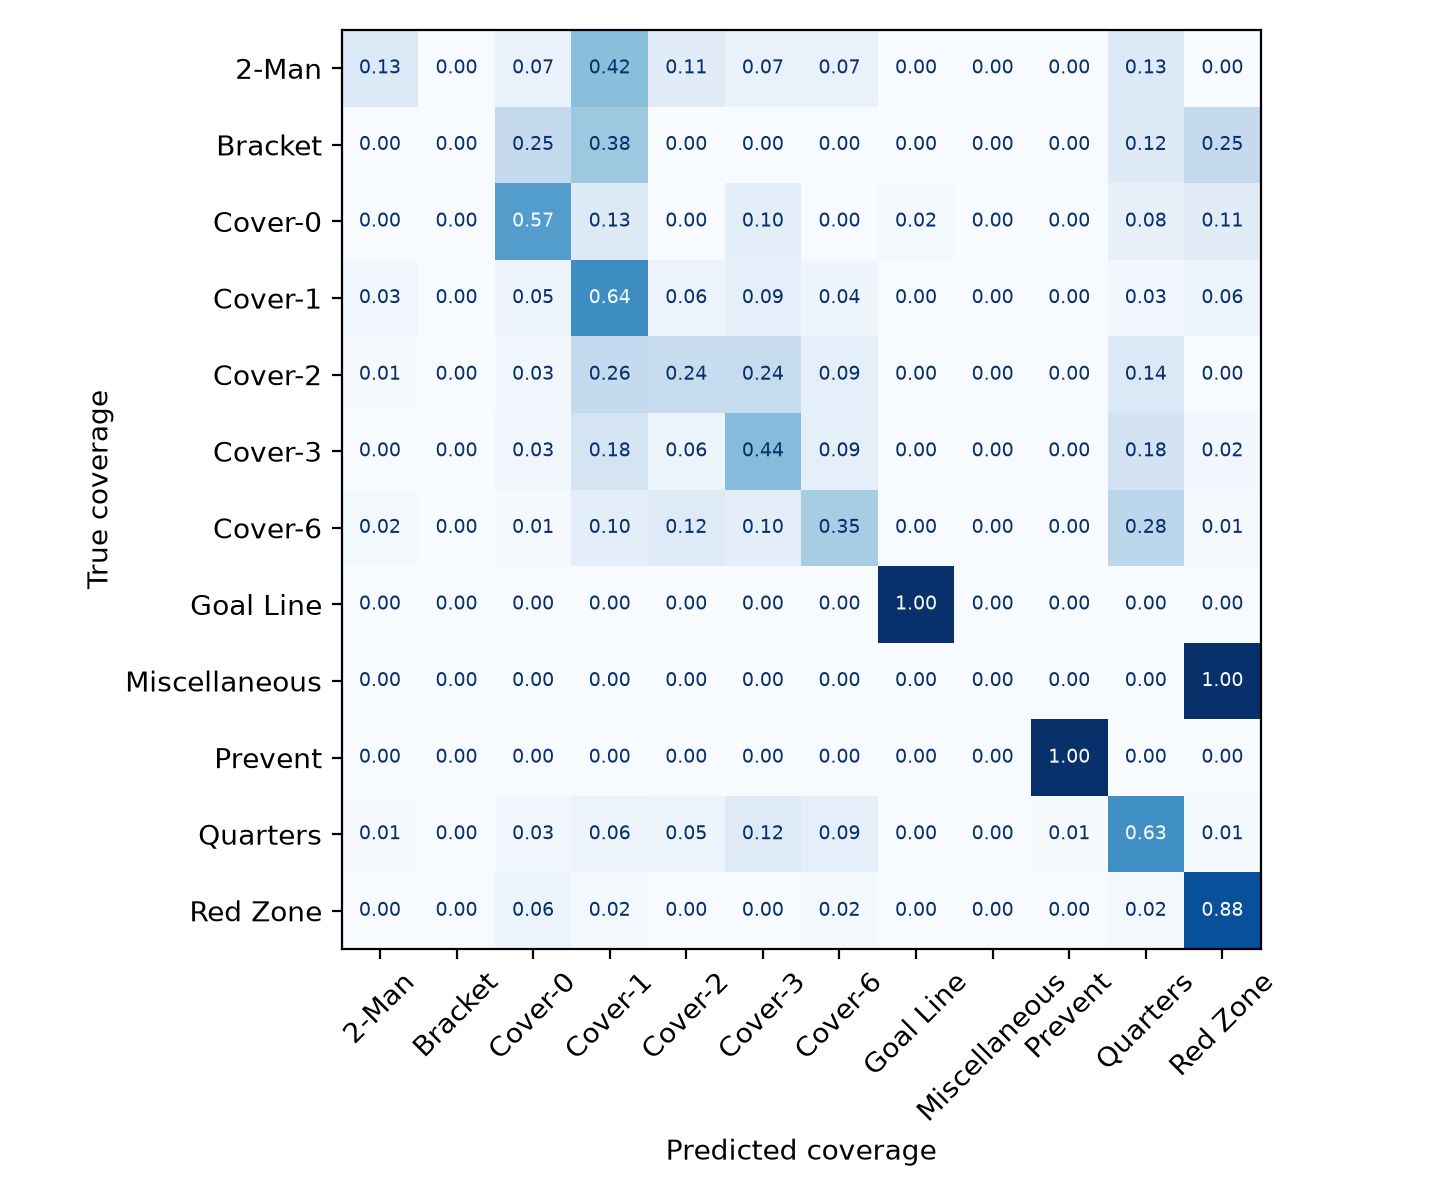
\includegraphics[width=0.62\textwidth]{confusion_matrix.png}
  \caption{\label{fig:confusion}Normalized confusion matrix on the validation split (each row sums to 1). Rows are true coverages and columns are predictions.}
\end{figure*}

\section{Feedback and Plans}

We met with our TA, Shreya Banik, who said that our data and model look good and that our planned next steps are sensible. These were grouped 5-fold cross-validation, experimenting with other models such as XGBoost and gradient boosting, and adding player roles as a feature. She also suggested optimizing accuracy per class, and she asked us to justify our design choices, such as our choice of model. We added that justification in Section~5.

She had reservations about combining all of the classes with few games into one, because those coverages might contradict each other and make the combined class noisy. She suggested that, instead of merging them or keeping them separate, we could drop such classes completely if they contradict the other coverages. Based on her feedback we will not merge them. We will keep them for now, and decide with cross-validation whether to drop specific classes that cannot be learned or that conflict with the others.

Our plan for the remaining weeks, following her feedback and our own review of the results:
\begin{itemize}
  \item Replace the single 18-game validation split with grouped 5-fold cross-validation by game, so that estimates use all 122 games, and run the test set once at the end.
  \item Decide whether to drop the rare coverage classes (Bracket, Prevent, Goal Line, and Miscellaneous), using the cross-validated per-class results, and report results with and without them.
  \item Compare the Random Forest with gradient-boosted trees (XGBoost) under the same folds and features.
  \item Add player roles (such as safety and cornerback) from the player metadata, to replace our position-free geometry features with role-based ones.
  \item Evaluate and optimize performance per class, for example through class weights or per-class decision thresholds, and report per-class results alongside macro-F1.
  \item Test removing team names and replacing the absolute score gap with a signed score differential.
\end{itemize}
Our largest gain so far came from the alignment features, which supports the premise that pre-snap geometry carries real information about coverage.

\section*{Team Contributions}

Zayed Umer collected and audited the regional dataset. Justin Kwinecki built the cleaning pipeline, the alignment features, and the Random Forest training and benchmarks. William Pol wrote this report and reviewed and verified the trained model and code.

\bibliography{custom}

\end{document}
